\documentclass[12pt]{article}
\usepackage{graphics}
\begin{document}

\noindent
Name:\,\makebox[0.8\textwidth]{\hrulefill} \\
\textbf{Observational Astronomy midterm exam} \\
Wednesday 2007-03-21 \\
\resizebox{\textwidth}{!}{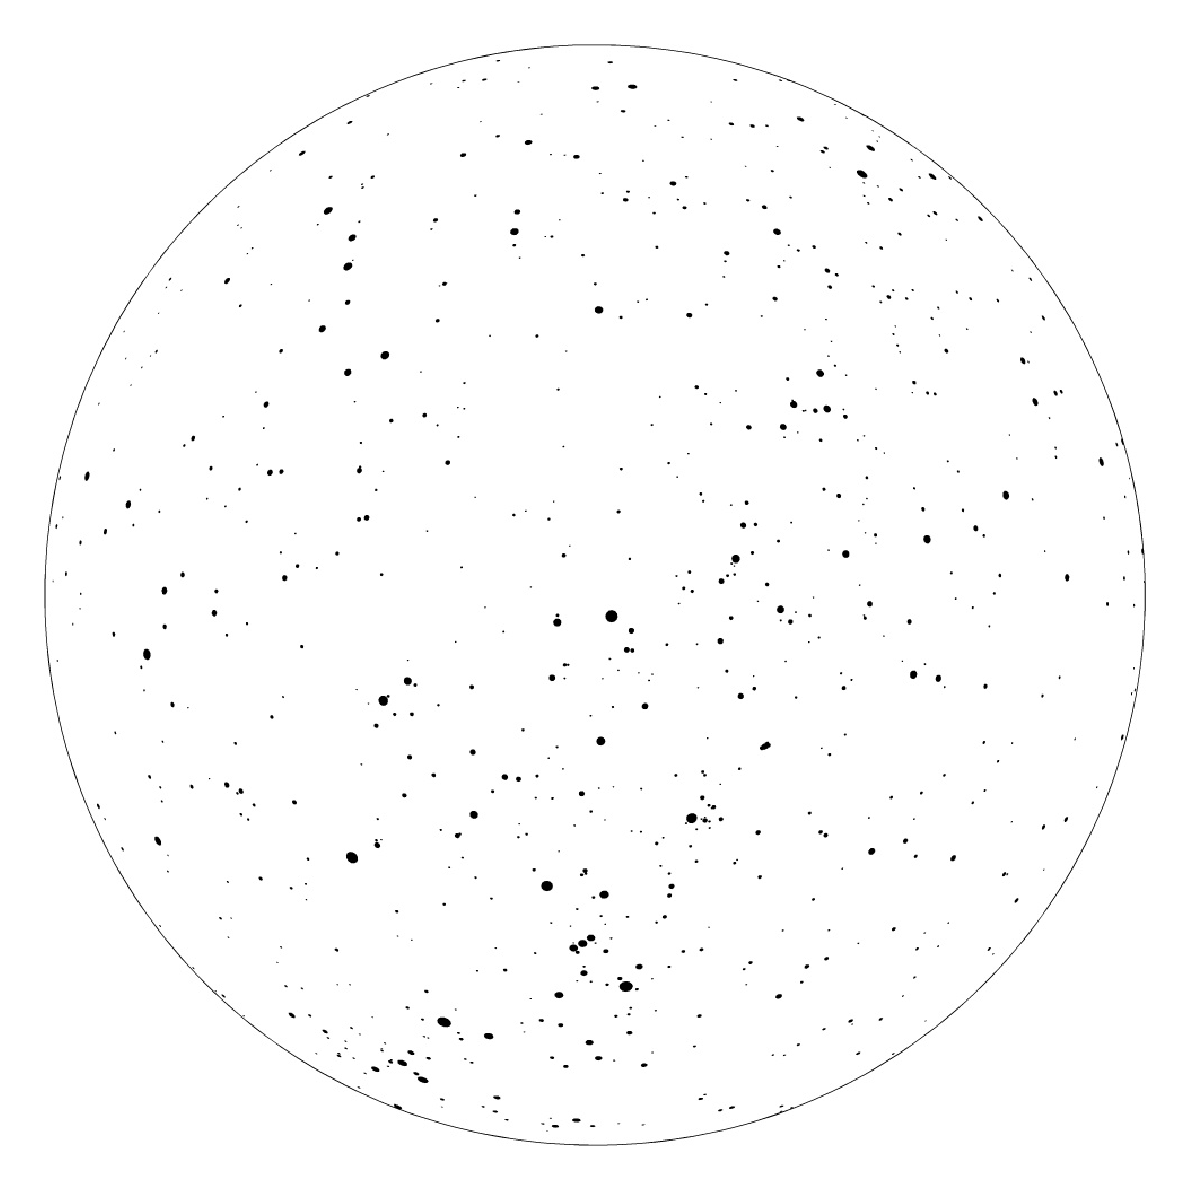
\includegraphics{chart_5_30.ps}}

\begin{enumerate}

\item
Above is an unlabeled map of the sky with the NYC zenith at the
center, appropriate for some night this semester.  \emph{Circle and
label} each of the following carefully and unambiguously:
\begin{itemize}
\item $\beta$ Ursa Majoris
\item $\alpha$ Cassiopeiae
\item Capella
\item the constellation Gemini
\item Rigel
\item RA=6\,hr, Dec=0\,deg (\emph{mark this point with a ``$+$''})
\item the constellation Crux
\end{itemize}
If any of these are not in the map, clearly write ``not in map''.
\emph{Note that the map is distorted at the edges; use your
judgement.}

\item
On the map, draw, as accurately as you can, the position Mars will
have in August 2007, according to the Field Guide.  Label Mars
unambiguously.

\item 
What is 1 min in arcmin?

\vspace{0.5in}

\item 
What is 1 deg in arcsec?

\vspace{0.5in}

\item 
Use your atlas to determine the RA and Dec of the star $\epsilon$ in
the constellation of Centaurus to within 10 min and 1 degree,
respectively.

\vspace{0.5in}

\item
Consider the stars $\alpha$, $\beta$, $\gamma$, $\delta$ in Capricorn.

Which of these four stars crosses the meridian first?

\vspace{0.5in}

As the Sun moves relative to the stars throughout the year, to which
of these four stars does the Sun come closest?

\vspace{0.5in}

\item 
In NYC tonight, at what altitude does Spica cross the meridian?

\vspace{0.5in}

\item
Explain how your answer to the previous question will depend on the
season.

\vspace{1in}

\item
In Havana, Cuba (lat=$+23.5$\,deg) tonight, at what altitude does
Spica cross the meridian?

\vspace{0.5in}

\item
Specify exactly the condition on the coordinates of a star that makes
it never visible for an observer on the Earth at latitude $\lambda$.

\vspace{1in}

\item
Circle all of the following that pass through the zenith in NYC at
some time during the year:
\begin{itemize}
\item the ecliptic
\item the Dec=55\,deg line
\item the celestial equator
\end{itemize}

\item 
You are at a latitude of $+30$\,deg on Earth and the sidereal time is
8\,h\,30\,m.

What RA, Dec is on the horizon, directly north?

\vspace{0.5in}

What RA, Dec is on the horizon, directly west?

\vspace{0.5in}

\item
In NYC, you see a bright star at az=105\,deg, alt=15\,deg. If you
re-observe the star 15\,min later,
\begin{itemize}
\item the az has increased/decreased (\emph{circle your answer})
\item the alt has increased/decreased
\end{itemize}

\item 
According to sidereal time, Aldebaran crosses the meridian
earlier/later/at the same time compared to the previous night
(\emph{circle your answer}).

According to civil time, Aldebaran crosses the meridian
earlier/later/at the same time compared to the previous night.

\item
If the Sun is in the constellation Cancer (check the atlas), what is
the season?

\vspace{0.5in}

\item
What constellation will the Sun enter next?

\vspace{0.5in}

\item
What is the sidereal time at noon today?

\vspace{0.5in}

What is the sidereal time at 8 am tomorrow morning?

\vspace{0.5in}

\item
Auckland, New Zealand is at a latitude of $-37$\,deg.  What are the
maximum and minimum altitudes of the Sun at noon (local time) in
Auckland during the year?

\vspace{1in}

\item
One can sometimes see the dark side of a crescent moon lit up faintly.
Where does this light originate and how did it get there?

\vspace{1in}

\item 
The moon's phase is new / full / 1st~quarter / 3rd~quarter immediately
prior to a waxing gibbous phase (\emph{circle your answer}).

\item
Draw a waning crescent moon as it appears in NY just after sunrise.
Shade in the unlit part.

\vspace{1.5in}

\item 
On one evening, the Moon is close to a bright star. On the following
evening the Moon is distant from the star by approximately
1 fist (at arms length) / one pinkie (at arms length) / 45\,deg / 90\,deg
to the E / W of the star (\emph{circle your answers}).

\item 
In NY, all the planets rise and set in a typical 24 hour period.  True
or false?

\vspace{0.5in}

\item 
A newly discovered planet in the Solar System has a nearly circular
orbit with orbital radius $0.64$\,AU.  What is it's sidereal period
in yr?  \emph{Show your work.}  Hint: $0.64=16/25$.

\vspace{1.5in}

\item
What is the ratio of the newly discovered planet's angular size (in,
say, arcmin) at inferior conjunction to its angular size at superior
conjunction?  \emph{Show your work.}

\vspace{1.5in}

\item 
Is Venus closer to the Earth when gibbous or when crescent?

\vspace{0.5in}

\item
Jupiter (whose orbital period is about 12 yr) was in opposition in May
2006, in the constellation of Libra.  When will it next be in
opposition?

\vspace{0.5in}

\item
Which planet would have a longer synodic period, one with a semi-major
axis of 1.1\,AU or one with a semi-major axis of 1.2\,AU?

\vspace{0.5in}

\item
We observe from 715 Broadway.  As you look downtown along Broadway, is
due South to your left or to your right?

\vspace{0.5in}

\end{enumerate}
\end{document}
